% GNUPLOT: LaTeX picture with Postscript
\begingroup
  \makeatletter
  \providecommand\color[2][]{%
    \GenericError{(gnuplot) \space\space\space\@spaces}{%
      Package color not loaded in conjunction with
      terminal option `colourtext'%
    }{See the gnuplot documentation for explanation.%
    }{Either use 'blacktext' in gnuplot or load the package
      color.sty in LaTeX.}%
    \renewcommand\color[2][]{}%
  }%
  \providecommand\includegraphics[2][]{%
    \GenericError{(gnuplot) \space\space\space\@spaces}{%
      Package graphicx or graphics not loaded%
    }{See the gnuplot documentation for explanation.%
    }{The gnuplot epslatex terminal needs graphicx.sty or graphics.sty.}%
    \renewcommand\includegraphics[2][]{}%
  }%
  \providecommand\rotatebox[2]{#2}%
  \@ifundefined{ifGPcolor}{%
    \newif\ifGPcolor
    \GPcolortrue
  }{}%
  \@ifundefined{ifGPblacktext}{%
    \newif\ifGPblacktext
    \GPblacktexttrue
  }{}%
  % define a \g@addto@macro without @ in the name:
  \let\gplgaddtomacro\g@addto@macro
  % define empty templates for all commands taking text:
  \gdef\gplbacktext{}%
  \gdef\gplfronttext{}%
  \makeatother
  \ifGPblacktext
    % no textcolor at all
    \def\colorrgb#1{}%
    \def\colorgray#1{}%
  \else
    % gray or color?
    \ifGPcolor
      \def\colorrgb#1{\color[rgb]{#1}}%
      \def\colorgray#1{\color[gray]{#1}}%
      \expandafter\def\csname LTw\endcsname{\color{white}}%
      \expandafter\def\csname LTb\endcsname{\color{black}}%
      \expandafter\def\csname LTa\endcsname{\color{black}}%
      \expandafter\def\csname LT0\endcsname{\color[rgb]{1,0,0}}%
      \expandafter\def\csname LT1\endcsname{\color[rgb]{0,1,0}}%
      \expandafter\def\csname LT2\endcsname{\color[rgb]{0,0,1}}%
      \expandafter\def\csname LT3\endcsname{\color[rgb]{1,0,1}}%
      \expandafter\def\csname LT4\endcsname{\color[rgb]{0,1,1}}%
      \expandafter\def\csname LT5\endcsname{\color[rgb]{1,1,0}}%
      \expandafter\def\csname LT6\endcsname{\color[rgb]{0,0,0}}%
      \expandafter\def\csname LT7\endcsname{\color[rgb]{1,0.3,0}}%
      \expandafter\def\csname LT8\endcsname{\color[rgb]{0.5,0.5,0.5}}%
    \else
      % gray
      \def\colorrgb#1{\color{black}}%
      \def\colorgray#1{\color[gray]{#1}}%
      \expandafter\def\csname LTw\endcsname{\color{white}}%
      \expandafter\def\csname LTb\endcsname{\color{black}}%
      \expandafter\def\csname LTa\endcsname{\color{black}}%
      \expandafter\def\csname LT0\endcsname{\color{black}}%
      \expandafter\def\csname LT1\endcsname{\color{black}}%
      \expandafter\def\csname LT2\endcsname{\color{black}}%
      \expandafter\def\csname LT3\endcsname{\color{black}}%
      \expandafter\def\csname LT4\endcsname{\color{black}}%
      \expandafter\def\csname LT5\endcsname{\color{black}}%
      \expandafter\def\csname LT6\endcsname{\color{black}}%
      \expandafter\def\csname LT7\endcsname{\color{black}}%
      \expandafter\def\csname LT8\endcsname{\color{black}}%
    \fi
  \fi
  \setlength{\unitlength}{0.0500bp}%
  \begin{picture}(8206.00,13680.00)%
      \csname LTb\endcsname%
      \put(4103,13460){\makebox(0,0){\strut{}Referenzspektren Teil 2}}%
    \gplgaddtomacro\gplbacktext{%
      \csname LTb\endcsname%
      \put(688,9234){\makebox(0,0)[r]{\strut{}0}}%
      \csname LTb\endcsname%
      \put(688,9986){\makebox(0,0)[r]{\strut{}2000}}%
      \csname LTb\endcsname%
      \put(688,10738){\makebox(0,0)[r]{\strut{}4000}}%
      \csname LTb\endcsname%
      \put(688,11491){\makebox(0,0)[r]{\strut{}6000}}%
      \csname LTb\endcsname%
      \put(688,12243){\makebox(0,0)[r]{\strut{}8000}}%
      \csname LTb\endcsname%
      \put(688,12995){\makebox(0,0)[r]{\strut{}10000}}%
      \csname LTb\endcsname%
      \put(820,9014){\makebox(0,0){\strut{} }}%
      \csname LTb\endcsname%
      \put(1462,9014){\makebox(0,0){\strut{} }}%
      \csname LTb\endcsname%
      \put(2105,9014){\makebox(0,0){\strut{} }}%
      \csname LTb\endcsname%
      \put(2747,9014){\makebox(0,0){\strut{} }}%
      \csname LTb\endcsname%
      \put(3389,9014){\makebox(0,0){\strut{} }}%
      \csname LTb\endcsname%
      \put(4031,9014){\makebox(0,0){\strut{} }}%
      \put(-214,11114){\rotatebox{-270}{\makebox(0,0){\strut{}Counts}}}%
      \put(3839,12694){\makebox(0,0)[l]{\strut{}Ag}}%
    }%
    \gplgaddtomacro\gplfronttext{%
    }%
    \gplgaddtomacro\gplbacktext{%
      \csname LTb\endcsname%
      \put(3971,9234){\makebox(0,0)[r]{\strut{}}}%
      \csname LTb\endcsname%
      \put(3971,9986){\makebox(0,0)[r]{\strut{}}}%
      \csname LTb\endcsname%
      \put(3971,10738){\makebox(0,0)[r]{\strut{}}}%
      \csname LTb\endcsname%
      \put(3971,11491){\makebox(0,0)[r]{\strut{}}}%
      \csname LTb\endcsname%
      \put(3971,12243){\makebox(0,0)[r]{\strut{}}}%
      \csname LTb\endcsname%
      \put(3971,12995){\makebox(0,0)[r]{\strut{}}}%
      \csname LTb\endcsname%
      \put(4103,9014){\makebox(0,0){\strut{} }}%
      \csname LTb\endcsname%
      \put(4745,9014){\makebox(0,0){\strut{} }}%
      \csname LTb\endcsname%
      \put(5387,9014){\makebox(0,0){\strut{} }}%
      \csname LTb\endcsname%
      \put(6029,9014){\makebox(0,0){\strut{} }}%
      \csname LTb\endcsname%
      \put(6671,9014){\makebox(0,0){\strut{} }}%
      \csname LTb\endcsname%
      \put(7313,9014){\makebox(0,0){\strut{} }}%
      \put(7122,12694){\makebox(0,0)[l]{\strut{}Ti}}%
    }%
    \gplgaddtomacro\gplfronttext{%
    }%
    \gplgaddtomacro\gplbacktext{%
      \csname LTb\endcsname%
      \put(688,5130){\makebox(0,0)[r]{\strut{}0}}%
      \csname LTb\endcsname%
      \put(688,5882){\makebox(0,0)[r]{\strut{}2000}}%
      \csname LTb\endcsname%
      \put(688,6634){\makebox(0,0)[r]{\strut{}4000}}%
      \csname LTb\endcsname%
      \put(688,7387){\makebox(0,0)[r]{\strut{}6000}}%
      \csname LTb\endcsname%
      \put(688,8139){\makebox(0,0)[r]{\strut{}8000}}%
      \csname LTb\endcsname%
      \put(688,8891){\makebox(0,0)[r]{\strut{}10000}}%
      \csname LTb\endcsname%
      \put(820,4910){\makebox(0,0){\strut{} }}%
      \csname LTb\endcsname%
      \put(1462,4910){\makebox(0,0){\strut{} }}%
      \csname LTb\endcsname%
      \put(2105,4910){\makebox(0,0){\strut{} }}%
      \csname LTb\endcsname%
      \put(2747,4910){\makebox(0,0){\strut{} }}%
      \csname LTb\endcsname%
      \put(3389,4910){\makebox(0,0){\strut{} }}%
      \csname LTb\endcsname%
      \put(4031,4910){\makebox(0,0){\strut{} }}%
      \put(-214,7010){\rotatebox{-270}{\makebox(0,0){\strut{}Counts}}}%
      \put(3839,8590){\makebox(0,0)[l]{\strut{}W}}%
    }%
    \gplgaddtomacro\gplfronttext{%
    }%
    \gplgaddtomacro\gplbacktext{%
      \csname LTb\endcsname%
      \put(3971,5130){\makebox(0,0)[r]{\strut{}}}%
      \csname LTb\endcsname%
      \put(3971,5882){\makebox(0,0)[r]{\strut{}}}%
      \csname LTb\endcsname%
      \put(3971,6634){\makebox(0,0)[r]{\strut{}}}%
      \csname LTb\endcsname%
      \put(3971,7387){\makebox(0,0)[r]{\strut{}}}%
      \csname LTb\endcsname%
      \put(3971,8139){\makebox(0,0)[r]{\strut{}}}%
      \csname LTb\endcsname%
      \put(3971,8891){\makebox(0,0)[r]{\strut{}}}%
      \csname LTb\endcsname%
      \put(4103,4910){\makebox(0,0){\strut{} }}%
      \csname LTb\endcsname%
      \put(4745,4910){\makebox(0,0){\strut{} }}%
      \csname LTb\endcsname%
      \put(5387,4910){\makebox(0,0){\strut{} }}%
      \csname LTb\endcsname%
      \put(6029,4910){\makebox(0,0){\strut{} }}%
      \csname LTb\endcsname%
      \put(6671,4910){\makebox(0,0){\strut{} }}%
      \csname LTb\endcsname%
      \put(7313,4910){\makebox(0,0){\strut{} }}%
      \put(7122,8590){\makebox(0,0)[l]{\strut{}Sn}}%
    }%
    \gplgaddtomacro\gplfronttext{%
    }%
    \gplgaddtomacro\gplbacktext{%
      \csname LTb\endcsname%
      \put(688,1025){\makebox(0,0)[r]{\strut{}0}}%
      \csname LTb\endcsname%
      \put(688,1777){\makebox(0,0)[r]{\strut{}2000}}%
      \csname LTb\endcsname%
      \put(688,2530){\makebox(0,0)[r]{\strut{}4000}}%
      \csname LTb\endcsname%
      \put(688,3282){\makebox(0,0)[r]{\strut{}6000}}%
      \csname LTb\endcsname%
      \put(688,4035){\makebox(0,0)[r]{\strut{}8000}}%
      \csname LTb\endcsname%
      \put(688,4787){\makebox(0,0)[r]{\strut{}10000}}%
      \csname LTb\endcsname%
      \put(820,805){\makebox(0,0){\strut{} }}%
      \csname LTb\endcsname%
      \put(1462,805){\makebox(0,0){\strut{} }}%
      \csname LTb\endcsname%
      \put(2105,805){\makebox(0,0){\strut{} }}%
      \csname LTb\endcsname%
      \put(2747,805){\makebox(0,0){\strut{} }}%
      \csname LTb\endcsname%
      \put(3389,805){\makebox(0,0){\strut{} }}%
      \csname LTb\endcsname%
      \put(4031,805){\makebox(0,0){\strut{} }}%
      \put(-214,2906){\rotatebox{-270}{\makebox(0,0){\strut{}Counts}}}%
      \put(2461,475){\makebox(0,0){\strut{}x}}%
      \put(3839,4486){\makebox(0,0)[l]{\strut{}Zn}}%
    }%
    \gplgaddtomacro\gplfronttext{%
    }%
    \gplgaddtomacro\gplbacktext{%
      \csname LTb\endcsname%
      \put(3971,1025){\makebox(0,0)[r]{\strut{}}}%
      \csname LTb\endcsname%
      \put(3971,1777){\makebox(0,0)[r]{\strut{}}}%
      \csname LTb\endcsname%
      \put(3971,2530){\makebox(0,0)[r]{\strut{}}}%
      \csname LTb\endcsname%
      \put(3971,3282){\makebox(0,0)[r]{\strut{}}}%
      \csname LTb\endcsname%
      \put(3971,4035){\makebox(0,0)[r]{\strut{}}}%
      \csname LTb\endcsname%
      \put(3971,4787){\makebox(0,0)[r]{\strut{}}}%
      \csname LTb\endcsname%
      \put(4103,805){\makebox(0,0){\strut{} }}%
      \csname LTb\endcsname%
      \put(4745,805){\makebox(0,0){\strut{} }}%
      \csname LTb\endcsname%
      \put(5387,805){\makebox(0,0){\strut{} }}%
      \csname LTb\endcsname%
      \put(6029,805){\makebox(0,0){\strut{} }}%
      \csname LTb\endcsname%
      \put(6671,805){\makebox(0,0){\strut{} }}%
      \csname LTb\endcsname%
      \put(7313,805){\makebox(0,0){\strut{} }}%
      \put(5743,475){\makebox(0,0){\strut{}x}}%
      \put(7122,4486){\makebox(0,0)[l]{\strut{}Zr}}%
    }%
    \gplgaddtomacro\gplfronttext{%
    }%
    \gplbacktext
    \put(0,0){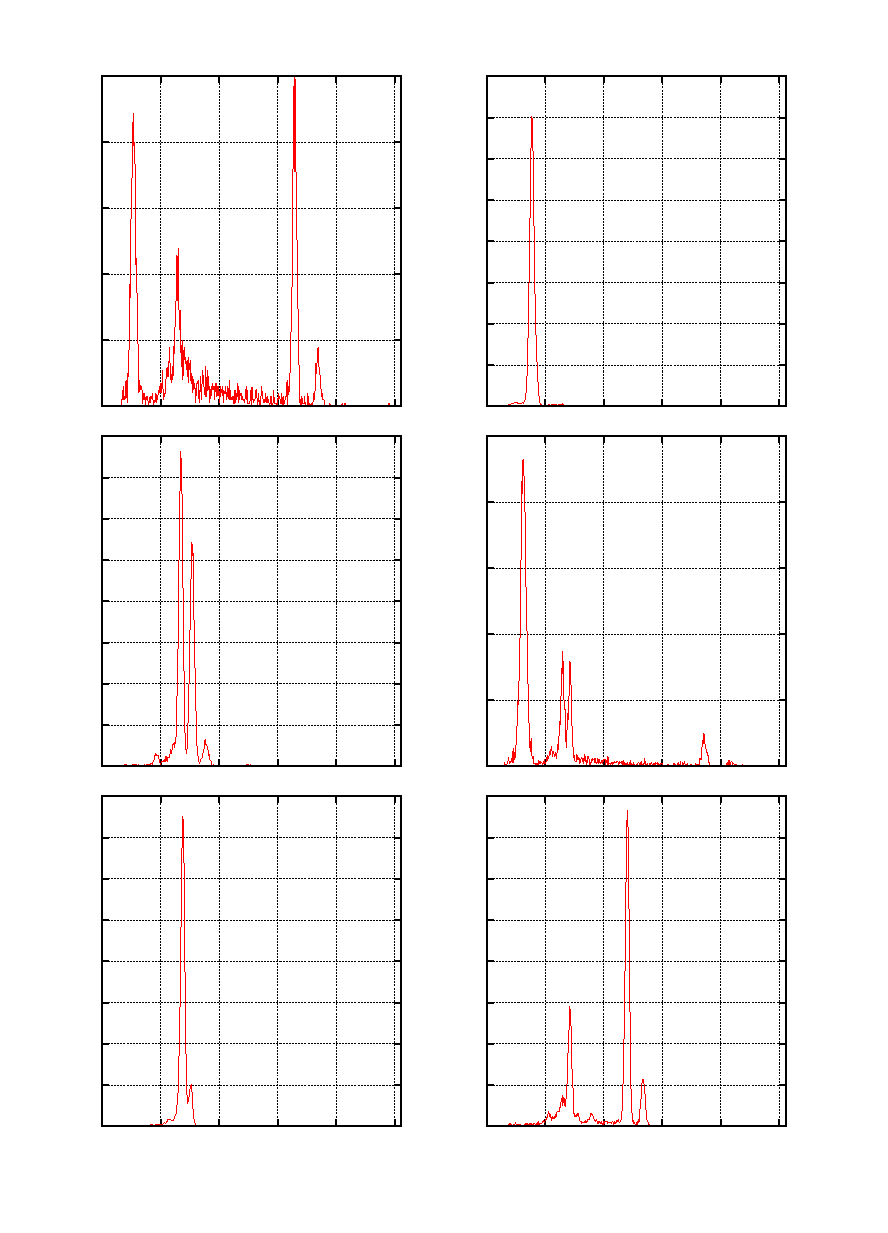
\includegraphics{./plots/referenzspektren2}}%
    \gplfronttext
  \end{picture}%
\endgroup
